\chapter{Biometria}
\label{cp:cap2}
Este capítulo possui como objetivo principal apresentar conceitos fundamentais da biometria, algumas modalidades biométricas, e principalmente a biometria de face e seus cenários, de modo a possibilitar um maior embasamento para compreensão da pesquisa.  Paralelamente apresenta-se os ambientes controlados e não controlados como também suas vantagens e eventuais desvantagens. 

\section{Características biométricas}


O emprego de características biométricas para identificação de pessoas teve suas primeiras ocorrências em meados do século XIX. Segundo \citeonline{costa2011ensemble}, o departamento de polícia de Paris foi o primeiro a utilizar formas de identificação de criminosos por meio da medição dos corpos. Pouco tempo depois descobriu-se que a impressão digital fornece características capazes de identificar um indivíduo \cite{jain2004introduction}. A partir desse marco temporal do surgimento da biometria, emergiram inúmeras iniciativas de modalidades biométricas.

A biometria surge perante a sociedade atual como uma alternativa aos  métodos de segurança tradicionais \cite{sharif2012survey}, os quais são propícios a fraudes e roubos. Mediante justificativas como esta, inúmeros órgãos públicos e privados vêm implantando medidas preventivas de segurança. Um destes órgãos é a polícia, que vem utilizando impressões digitais há décadas. A biometria é aplicada em inúmeras áreas, as quais podemos dividir em três grupos principais, a saber:
\begin{itemize}
\item Comercial, com o intuito de  promover, por exemplo, segurança nos cartões de crédito e restrição de acesso aos dispositivos móveis.
\item Governamental, cujo interesse é estabelecer normas de segurança em ambientes públicos visando favorecer toda a população.
\item Forense, tem como finalidade estratégias criminais, como por exemplo identificação de atitudes terroristas.
\end{itemize}
\section{Sistemas biométricos}
O processo de identificação biométrica pode ser dividido nas seguintes etapas: aquisição/segmentação, extração/seleção de características, comparação de características e armazenamento \cite{sharif2012survey}. Ultimamente a área de reconhecimento biométrico sofreu grandes avanços significativos em termos de confiabilidade e precisão. Segundo \citeonline{lone2011automatic}, algumas modalidades biométricas têm alcançado um bom desempenho em aplicações práticas. Dentre as principais modalidades biométricas temos: impressão digital, face \cite{sharif2012survey,[20]shermina2012recognition}, voz, palma da mão e íris.
Para que uma característica física ou comportamental de um ser humano possa ser vista como uma modalidade biométrica é necessário que alguns requisitos sejam satisfeitos \cite{jain2004introduction}:

\begin{itemize}
\item universalidade: cada pessoa deve possuir essa característica;
\item distinção: duas pessoas devem possuir características distintas;
\item permanência: a característica deve ser suficientemente constante (no que diz respeito ao critério de correspondência) durante um determinado período de tempo; 
\item mensurabilidade: deve ser possível medi-la. 
\end{itemize}
Segundo \citeonline{delac2004survey} um sistema biométrico é composto por um conjunto de módulos como pode ser visto na figura \ref{fig:modulos}.
\begin{itemize}
\item módulo Sensorial: módulo responsável por fazer a coleta da característica biométrica;
\item módulo de Extração das características: responsável por extrair as características que serão utilizadas para a construção do vetor de características;
\item módulo de Comparação: módulo responsável por realizar a comparação do vetor de características construído com os padrões armazenados na base de dados;
\item módulo de Decisão: responsável por verificar o retorno do módulo de comparação e decidir se o usuário com aquelas características é aceito ou não;
\item base de Dados: realiza o armazenamento de todos os padrões de usuários que irão fazer uso do sistema e disponibiliza essas informações para o módulo de comparação.
\end{itemize}

\begin{figure}[H]
\centering
\caption{Módulos de um sistema biométrico}
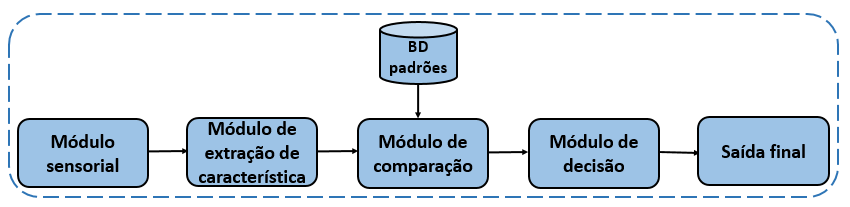
\includegraphics[scale = 0.66]{imgs3/modulos_biometria.png}
\source{Jonas Mendonça Targino, 2018}
\label{fig:modulos}
\end{figure}

Para o reconhecimento de uma pessoa é necessário o armazenamento prévio das suas características biométricas. Essa fase também chamada de cadastramento é anterior a fase de autenticação. Na etapa de autenticação existem dois modos: a identificação e a verificação, estas duas modalidades apresentam algumas diferenças no método envolvido, devido à natureza diferente de ambos.
\begin{itemize}
\item \textbf{Identificação -} também chamada de reconhecimento, é uma etapa em que o usuário fornece suas características para o sistema, e este realiza uma comparação com todos os \textit{templates} da base de dados (1:n). Neste caso, o sistema é responsável pela tarefa de comparar e analisar qual a pessoa da base de dados possui aquelas características. De forma resumida a imagem de consulta será comparada com todas as imagens armazenadas, e uma decisão será tomada de modo a identificar a classe à qual imagem de entrada pertence. A vantagem da identificação é que a mesma elimina a necessidade de uso de senhas ou cartões. A figura \ref{fig:identificacao} mostra como é realizado o processo de reconhecimento facial.
 
\begin{figure}[H]
\centering
\caption{Identificação ou reconhecimento facial}
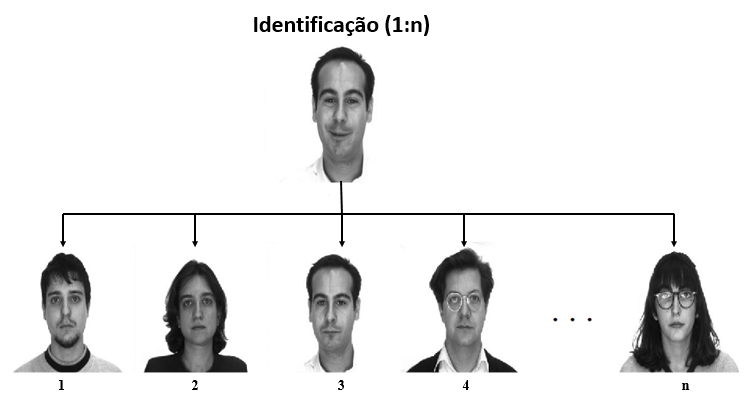
\includegraphics[scale = 0.75]{imgs/1praN.png}
\label{fig:identificacao}
\source{Jonas Mendonça Targino, 2018. Imagens de faces obtidas da base AR \cite{martinez1998ar}}
\end{figure}
 
\item \textbf{Verificação -} comumente chamada de autenticação, pode ser considerada um subconjunto da tarefa de reconhecimento. A etapa  de verificação envolve uma comparação um para um, entre a imagem de consulta e a imagem (ou classe) que o usuário afirma ser. Neste caso, o sistema recebe como entrada uma característica  e uma senha, este verifica se o usuário é a pessoa que alega ser. Em outras palavras, caso uma pessoa se posicionar na frente de um sistema como esse, e alegar ser uma determinada pessoa, o sistema irá analisar apenas se ela é aquele usuário que alega ser, ou não. A figura \ref{fig:verificacao} apresenta a etapa de autenticação.

\end{itemize}
\begin{figure}[H]
\centering
\caption{Verificação da face}
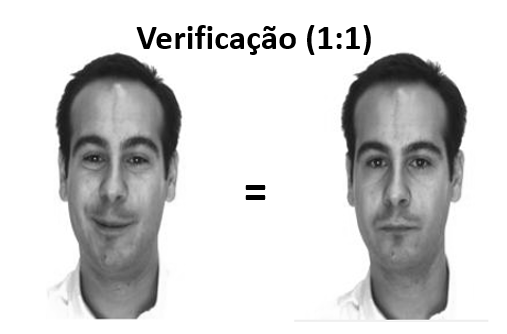
\includegraphics[scale = 0.50]{imgs/1pra1.png}
\label{fig:verificacao}
\source{Jonas Mendonça Targino, 2018. Imagens de faces obtidas da base AR \cite{martinez1998ar}}
\end{figure}


A figura \ref{fig:processo_ver_iden} ilustra um exemplo do processo de verificação e identificação, sendo possível perceber que na fase de verificação é retornado apenas 1 modelo (o qual o usuário afirma ser), já na fase de identificação são retornados todos os \textit{n} modelos presentes na base de dados.

\begin{figure}[H]
\centering
\caption{Exemplo do processo de verificação e identificação }
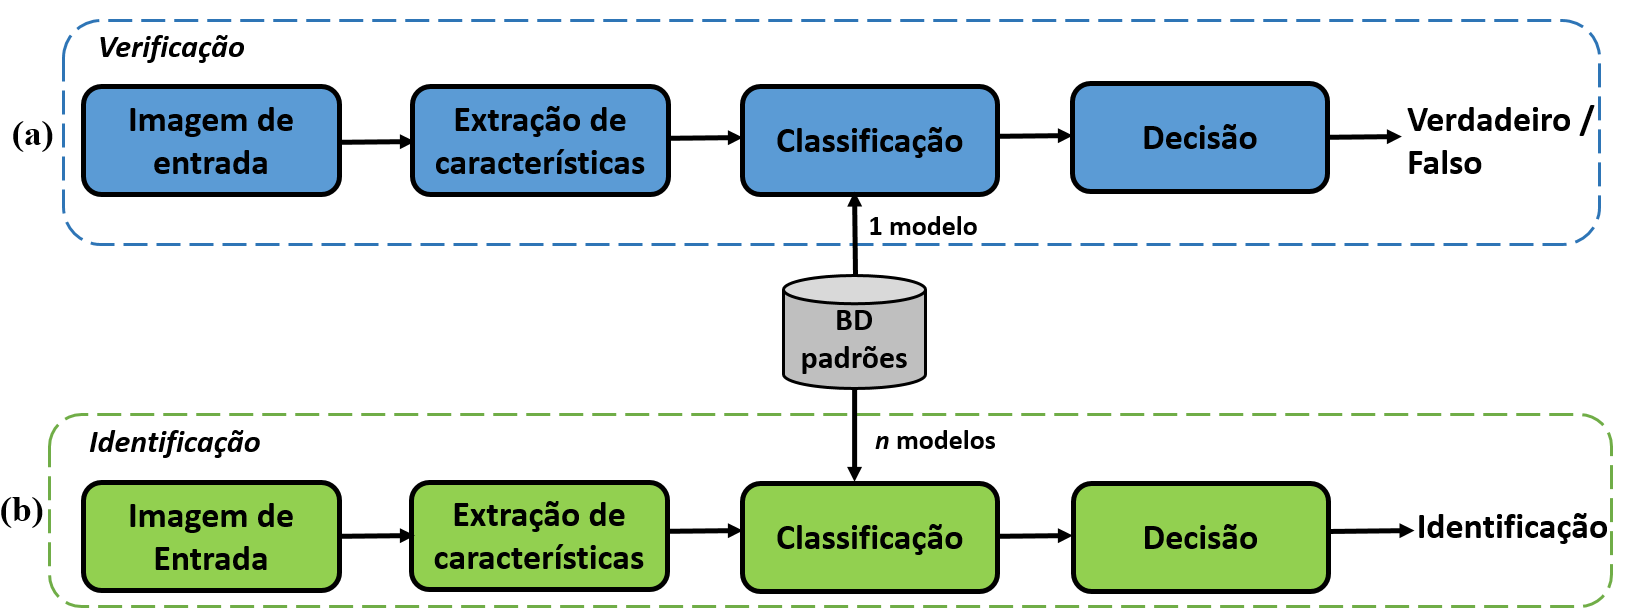
\includegraphics[scale = 0.33]{imgs3/verifi_identi}
\source{Jonas Mendonça Targino, 2018}
\label{fig:processo_ver_iden}
\end{figure}





\section{Modalidades biométricas}



Inúmeros trabalhos utilizam como estratégia de reconhecimento biométrico baseado em face, íris, impressão digital, palma de mão e forma de andar. Alguns destes trabalhos são os de \citeonline{galdi2016multimodal} e \citeonline{costa2011ensemble} que trabalham com íris com finalidades biométricas. O primeiro trabalho utiliza biometria multimodal realizando a combinação de íris e alguns sensores de reconhecimento com fins de identificação. Já o segundo trabalho utiliza a fusão de íris e face com fins biométricos alcançando resultados consideráveis perante a literatura, demonstrando com isso que a fusão de características biométricas é uma boa estratégia.

Já no contexto de impressão digital, o trabalho de \citeonline{Targino2018_wvc_duru} apresenta um estudo comparativo envolvendo técnicas tradicionais de classificação com cinco sensores, com iniciativas a mensurar qual o melhor sensor para extração das características. Paralelamente o trabalho de \citeonline{benaliouche2014comparative} também aborda o contexto de impressão digital combinando-a com íris objetivando obter melhores resultados em termos de reconhecimento, visto que a multimodalidade biométrica vem apresentando resultados significativos mediante o estado da arte.

Por outro lado, os trabalhos de \citeonline{kumar2017gait} e \citeonline{george2017efficient} utilizam a forma de andar como modalidade biométrica, de modo que os dois trabalhos atingiram resultados consideráveis de acurácia. De forma que o primeiro utilizou Máquina de Vetores Suporte (do inglês: \textit{Support Vector Machines} - SVM) e Redes Neurais Perceptron Multicamadas como classificadores. Já o segundo, utilizou apenas a rede neural como estratégia de classificação.

Com o auxílio da figura \ref{fig:exemplo_modalidades_biometricas} podemos visualizar oito exemplos de modalidades biométricas.


\begin{figure}[H]
\centering
\caption{Exemplos de algumas modalidades biométricas }
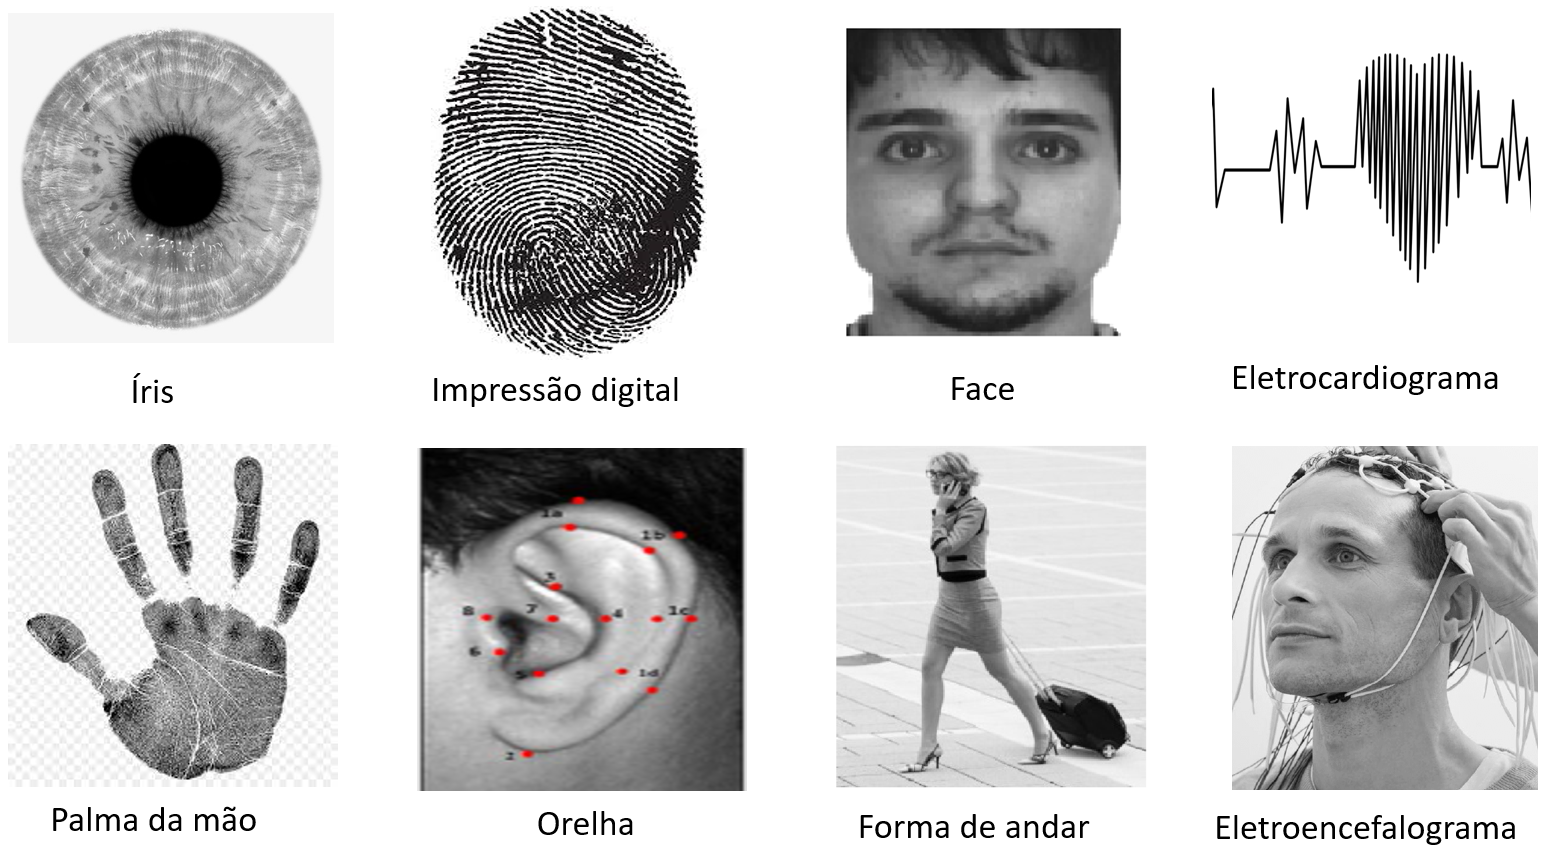
\includegraphics[scale = 0.38]{imgs3/modalidades_biometricas}
\source{Jonas Mendonça Targino, 2018}
\label{fig:exemplo_modalidades_biometricas}
\end{figure}






\section{Ambientes controlados versus não controlados}
\label{sec:amb. cont x n.cont}
Ambientes controlados são ambientes com condições propícias para a coleta de dados, projetados com esta finalidade. Já ambientes não controlados correspondem aos mais variados espaços, os quais podem fornecer uma coleta de dados, embora esta, não passe por um processo sistemático, o que possibilita amostras de dados ruidosas e consequentemente dificuldades de identificação do indivíduo. Considerando o contexto  de reconhecimento biométrico facial, ambientes controlados são locais com condições adequadas de iluminação, baixa complexidade de fundo da imagem, pequeno ângulo de visualização da câmera (geralmente em ambientes internos) e total colaboração do usuário junto ao sensor de coleta, de modo a evitar viés frente a captura da imagem a fim de minimizar seus efeitos na taxa de identificação do sistema. 

Em contrapartida ambientes não controlados são locais em que por questões de segurança, existe um sistema com câmeras de vídeo-vigilância com finalidade de identificar as pessoas presentes naquele determinado recinto (geralmente ambientes externos), de modo que as pessoas ali presentes estejam cientes que estão sendo filmadas. Em ambientes como este, o usuário não possui a menor intenção de colaborar frente a coleta de dados, como também não existe nenhuma preocupação em realizar um processo sistemático para a coleta de informações dos usuários presentes naquele local.